\section{Convolutional Network Trained on Synthetic Objects}
\label{sec:simple_cnn}

% cnn generalization results
\begin{figure*}[t]
    \begin{center}
        % subfigure (a)
        \begin{subfigure}[b]{0.48\textwidth}
            \begin{center}
                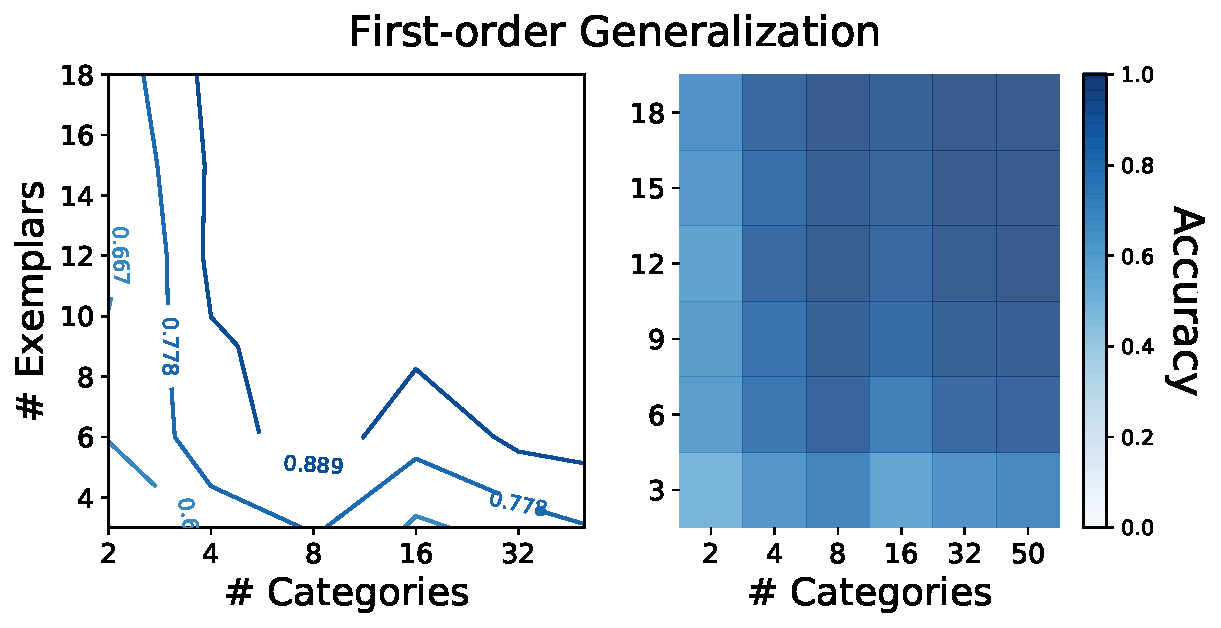
\includegraphics[width=0.98\textwidth]
                {figures/cnn_o1_acc.pdf}
            \end{center}
        \end{subfigure}
        % subfigure (b)
        \begin{subfigure}[b]{0.48\textwidth}
            \begin{center}
                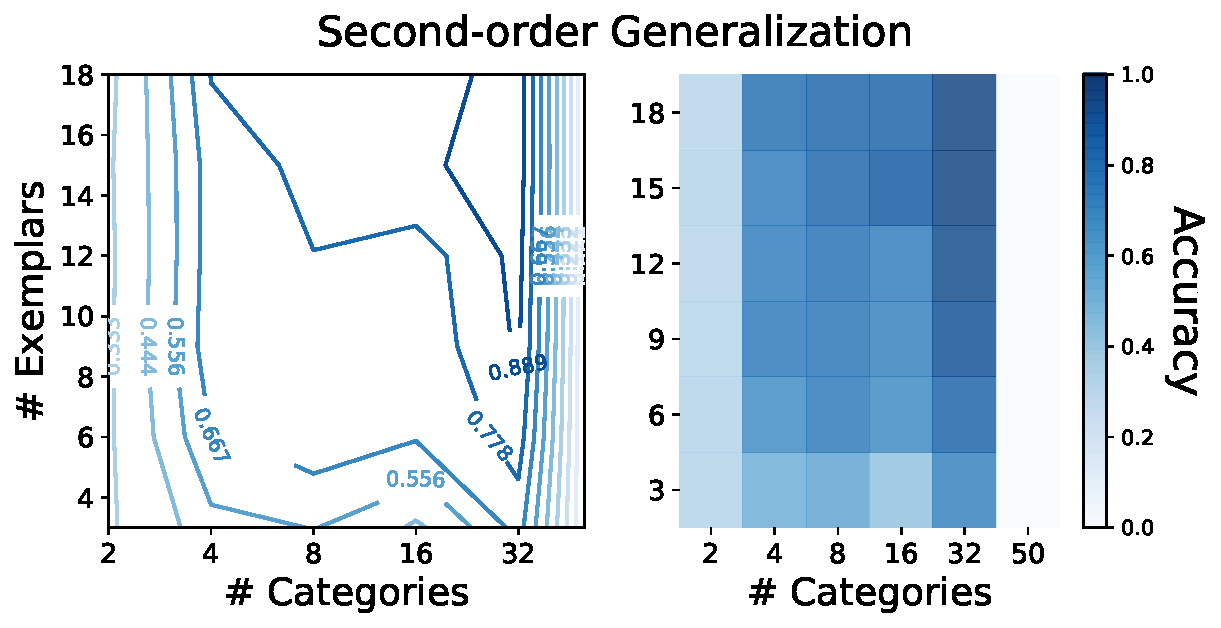
\includegraphics[width=0.98\textwidth]
                {figures/cnn_o2_acc.pdf}
            \end{center}
        \end{subfigure}
    \end{center}
    \caption{CNN generalization results for various training set sizes. Results
    show the average of 10 training runs.}
    \label{fig:cnn_gen_results}
\end{figure*}

Our first experiment uses a highly simplified data format. However, neural network
architectures can perform well with complex data, including natural
images, language and audio. In a successive experiment, ask whether similar
generalization results can be achieved using object stimuli encoded as RGB
images. To do so, we construct an image dataset consisting of artifical 2D
objects. Each object is a 2D shape of a specified color placed over white background.
Objects are initially centered, however, a random shift is applied to every sample.
Texture is represented in a fourth dimension, independent of RGB space. The motivation for this design choice
is as follows. In the experiments of \cite{Smith2002}, children physically touch
each object that they are presented in addition to observing it visually. Although the
presence of materials like plastic and styrofoam may be visually subtle compared
to color and shape, these materials become much more detectable when sensed by hand.
Since visual and touch signals are received along separate pathways, it makes
sense to provide these signals along independent axes to a computational model.

Object shapes are determined by randomly generating sets of points around the 2D
image window, and colors are generated to span the RGB vector space with even
separation. We use black \& white textures from the Brodatz database \citep{Brodatz1966}
for our texture categories. Some examples of our objects are shown in Fig.
\ref{fig:generated_images}. We train a convolutional neural network (CNN)
consisting of two convolution layers with five filters, each followed by a max pooling
layer. The last pooling layer is followed by a fully-connected layer of 25 ReLU
units, and the softmax layer again varies in size according to the number of
categories in the dataset. The initial second-order generalization results for a
random network are as follows: shape 0.39, color 0.41 and texture 0.20.
Results for networks trained on various dataset sizes are shown in Fig. \ref{fig:cnn_gen_results}.

We next analyze the parametric relationship between our CNN biases and the feature
values of presented stimuli similarly to our MLP. For our image objects,
distance in shape space is quantified as the Modified Hausdorff Distance
\citep{Dubuisson1994} between the shape pair. In color space, distance is
quantified using the cosine similarity of the RGB vector pair. The parametric
bias results are shown in Fig. \ref{fig:cnn_parametric}.

\begin{figure}[t!]
    \begin{center}
        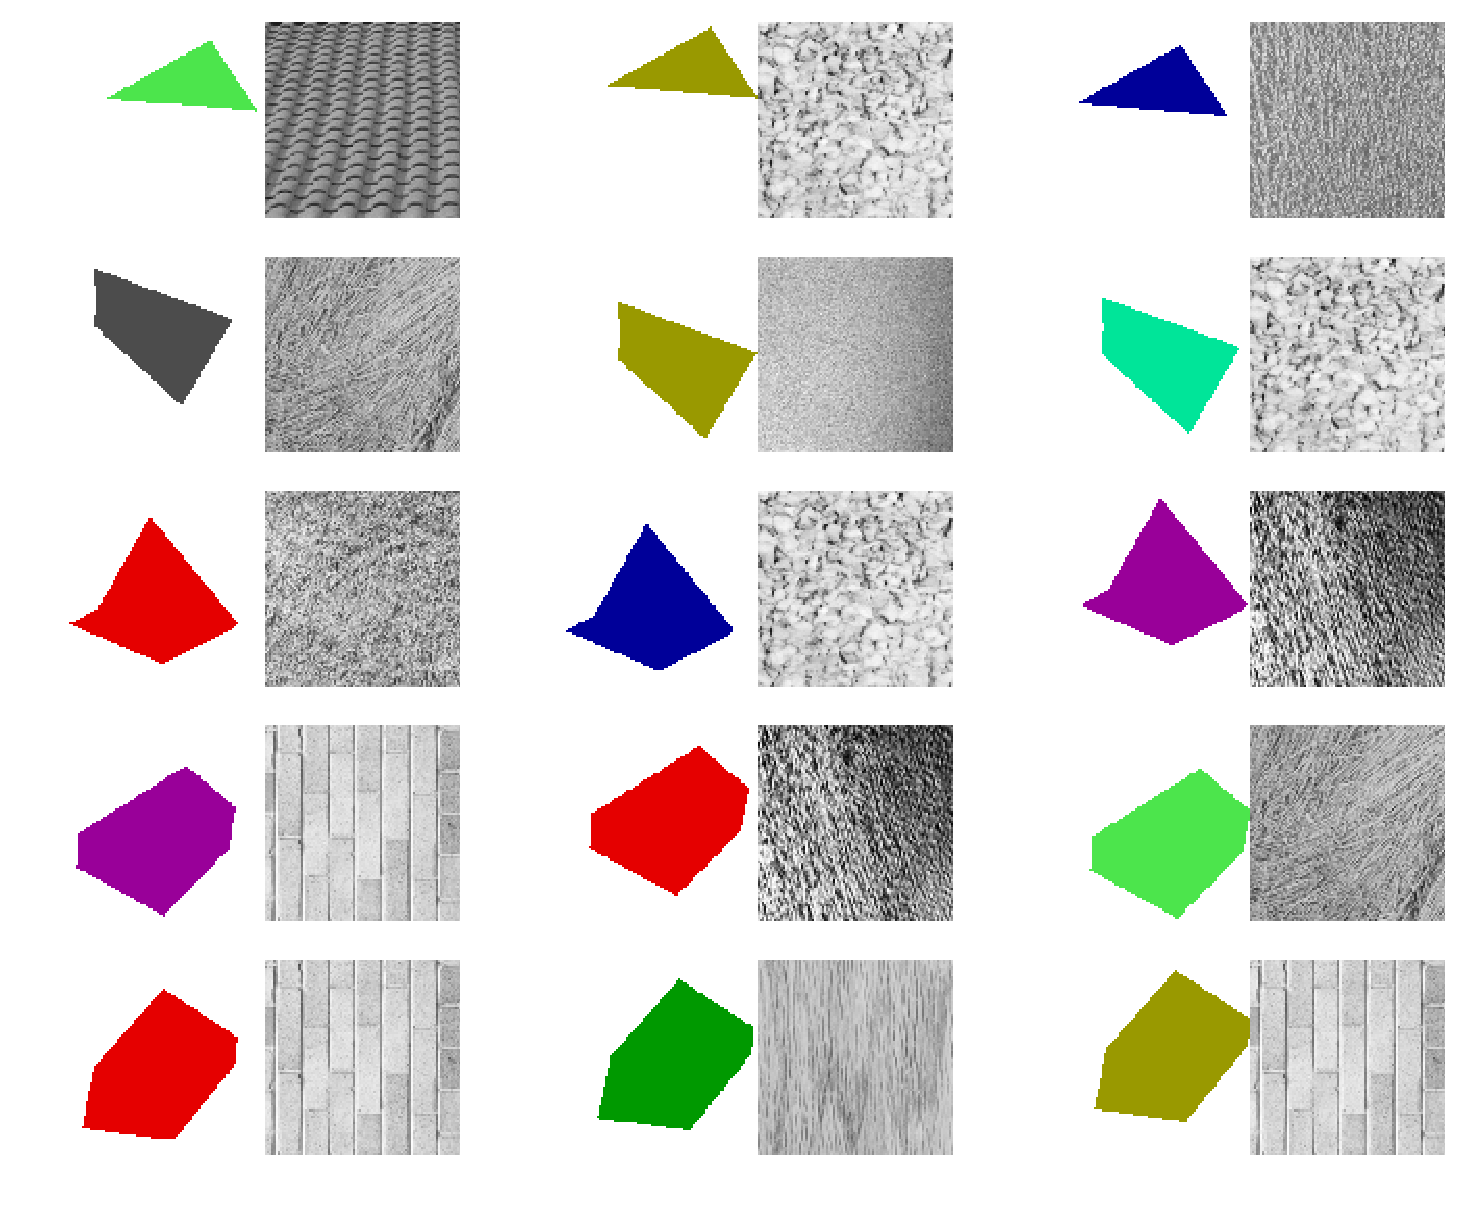
\includegraphics[width=0.45\textwidth]{figures/generated_images.pdf}
    \end{center}
    \caption{Computer-generated images of 2D objects with
    different shape, color and texture features. Rows correspond to object
    categories. Dimensions 1-3 are shown on the left of each image, and
    dimension 4 (texture) is shown on the right.}
    \label{fig:generated_images}
\end{figure}

\begin{figure}[h!]
    \begin{center}
        \begin{subfigure}[b]{0.235\textwidth}
            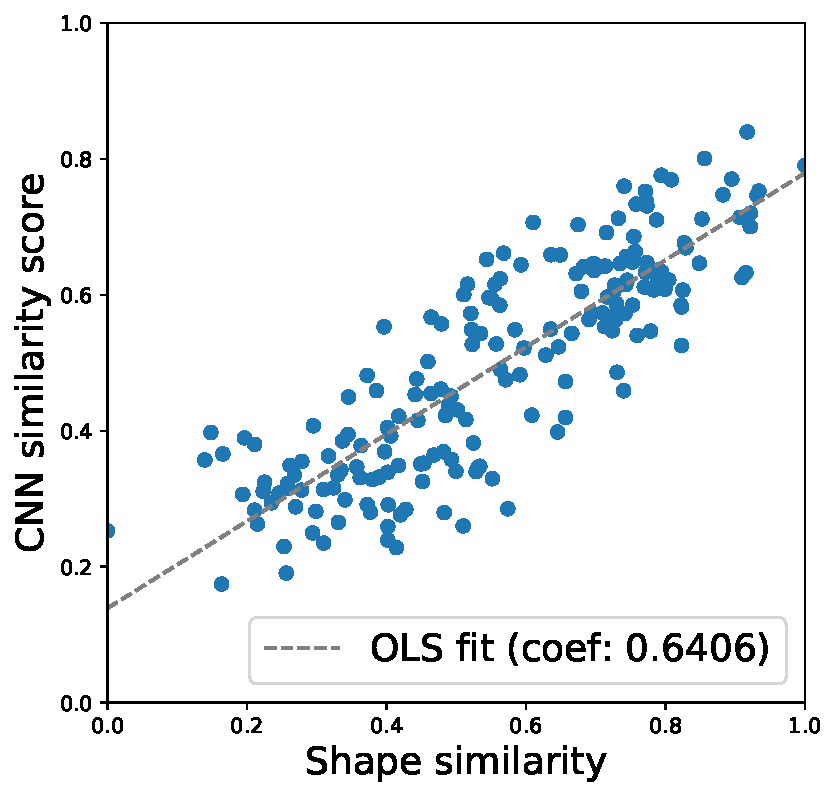
\includegraphics[width=\linewidth]
            {figures/vgg_shape_parametric_others_constant.pdf}
            \caption{Shape}
        \end{subfigure}
        \begin{subfigure}[b]{0.235\textwidth}
            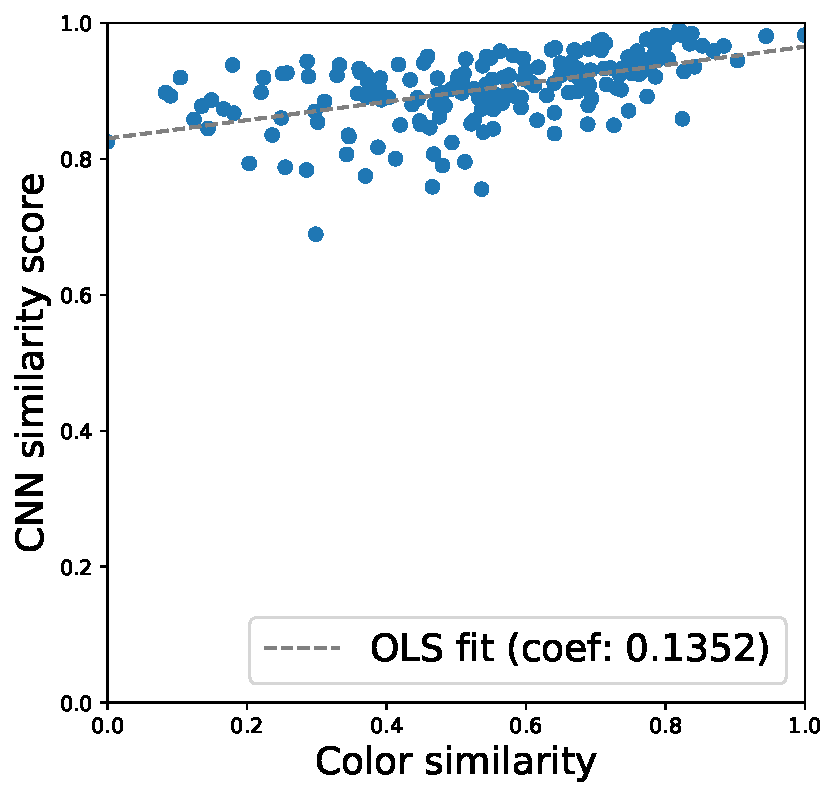
\includegraphics[width=\linewidth]
            {figures/vgg_color_parametric_others_constant.pdf}
            \caption{Color}
        \end{subfigure}
    \end{center}
    \caption{CNN parametric shape and color biases. TODO: put correct result
    plots here.}
    \label{fig:cnn_parametric}
\end{figure}

% \begin{figure}[h!]
%     \begin{center}
%         % shape 1
%         \begin{subfigure}[b]{0.15\textwidth}
%             \begin{center}
%                 \begin{subfigure}[b]{0.9\textwidth}
%                     \includegraphics[width=\linewidth]
%                     {figures/artist_objects/fake1_carpet_red.jpg}
%                 \end{subfigure}
%                 \begin{subfigure}[b]{0.9\textwidth}
%                     \includegraphics[width=\linewidth]
%                     {figures/artist_objects/fake1_sponge_yellow.jpg}
%                 \end{subfigure}
%             \end{center}
%         \end{subfigure}
%         % % shape 2
%         \begin{subfigure}[b]{0.15\textwidth}
%             \begin{center}
%                 \begin{subfigure}[b]{0.9\textwidth}
%                     \includegraphics[width=\linewidth]
%                     {figures/artist_objects/fake5_wood_pink.jpg}
%                 \end{subfigure}
%                 \begin{subfigure}[b]{0.9\textwidth}
%                     \includegraphics[width=\linewidth]
%                     {figures/artist_objects/fake5_carpet_purple.jpg}
%                 \end{subfigure}
%             \end{center}
%         \end{subfigure}
%         \begin{subfigure}[b]{0.15\textwidth}
%             \begin{center}
%                 \begin{subfigure}[b]{0.9\textwidth}
%                     \includegraphics[width=\linewidth]
%                     {figures/artist_objects/fake4_sponge_orange.jpg}
%                 \end{subfigure}
%                 \begin{subfigure}[b]{0.9\textwidth}
%                     \includegraphics[width=\linewidth]
%                     {figures/artist_objects/fake4_wood_green.jpg}
%                 \end{subfigure}
%             \end{center}
%         \end{subfigure}
%     \end{center}
%     \caption{Artist-designed images of 3D objects with different shape, color
%     and texture features.}
%     \label{fig:artist_images}
% \end{figure}

% \subsection{Layer-wise Biases}
% The first step of our analysis is to evaluate the shape, color and texture biases of VGG-16
% at each of its layers, in order to get a picture of how these biases develops along the
% higherarchy of the model's internal representation. In order to probe the model, we make
% use of two unique image datasets with stimuli that mimic \cite{Smith2002}.

% {\bf1. Artist-generated object dataset}: These images were generated by an artist in Adobe
% Photoshop. See Fig. \ref{fig:artist_images}.

% {\bf2. CogPsyc object dataset}: These images were provided by cognitive psychologist Linda
% Smith, and they were used in the experiments of \cite{Ritter2017}. See Fig.
% \ref{fig:cogpsyc_images}.

% \begin{figure*}[h]
%     \begin{center}
%         \begin{subfigure}[b]{0.4\textwidth}
%             \begin{center}
%                 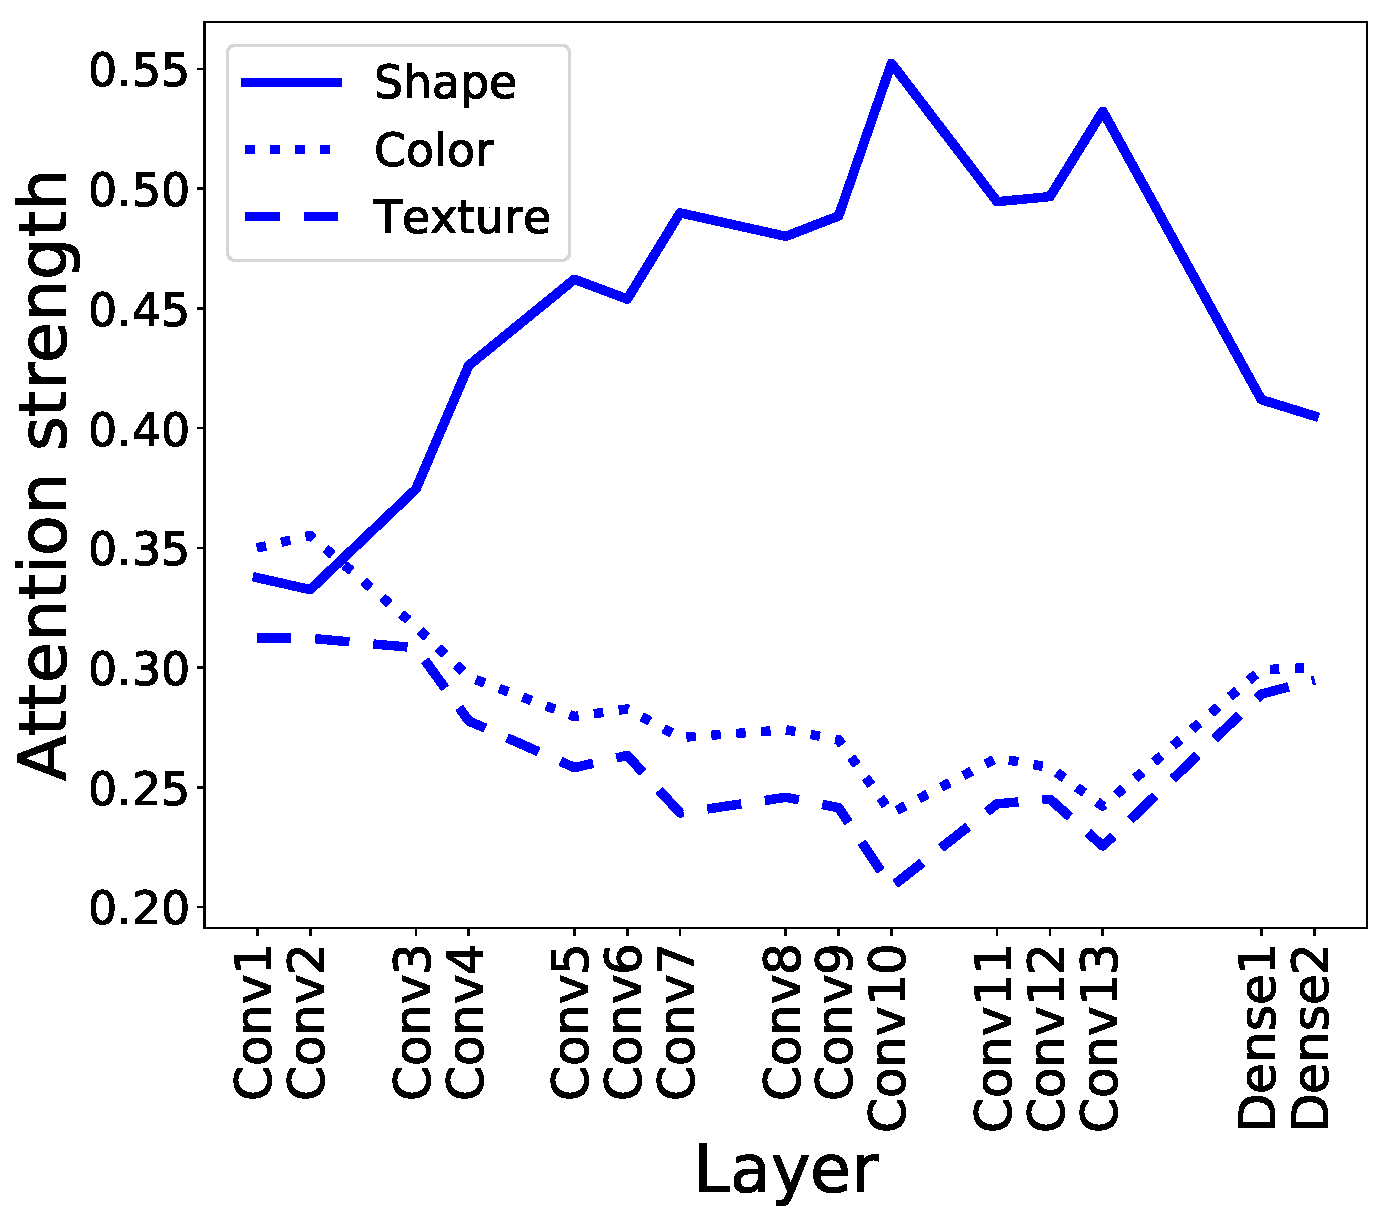
\includegraphics[width=\textwidth]{figures/vgg_layer_biases.pdf}
%             \end{center}
%             \caption{Artist-generated images}
%             \label{fig:biases_artist}
%         \end{subfigure}
%         \begin{subfigure}[b]{0.4\textwidth}
%             \caption{CogPsyc images (TODO)}
%         \end{subfigure}
%         \caption{VGG-16 layer-wise biases on two image datasets. Attention strength refers to
%         the network's similarity score between the target objectand objects that match in
%         either shape, color or texture.}
%     \end{center}
%     \label{fig:layerwise_biases}
% \end{figure*}

% \begin{figure}[h!]
%     \begin{center}
%         \begin{subfigure}[b]{0.235\textwidth}
%             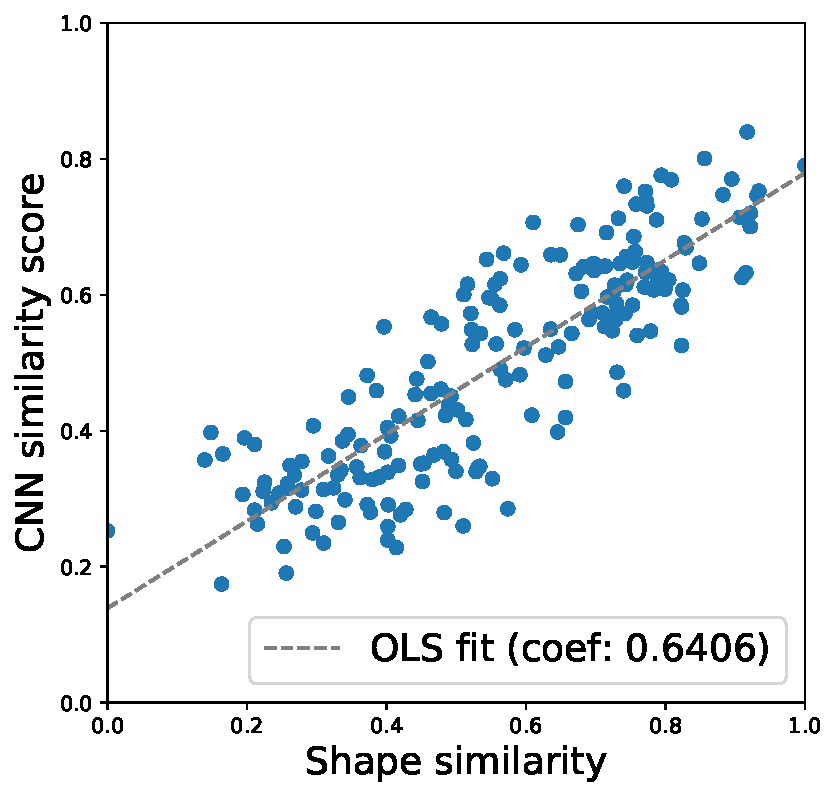
\includegraphics[width=\linewidth]{figures/vgg_shape_parametric_others_constant.pdf}
%             \caption{Shape}
%         \end{subfigure}
%         \begin{subfigure}[b]{0.235\textwidth}
%             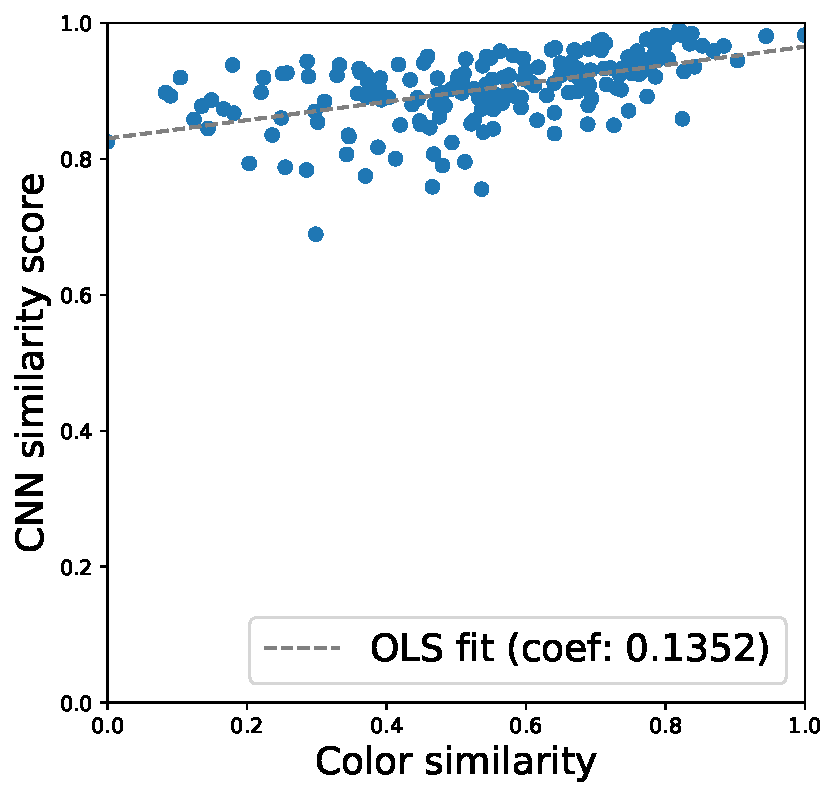
\includegraphics[width=\linewidth]{figures/vgg_color_parametric_others_constant.pdf}
%             \caption{Color}
%         \end{subfigure}
%     \end{center}
%     \caption{VGG-16 parametric shape and color biases w/ other features constant.}
%     \label{fig:parametric_others_constant}
% \end{figure}

% \begin{figure}[h!]
%     \begin{center}
%         \begin{subfigure}[b]{0.235\textwidth}
%             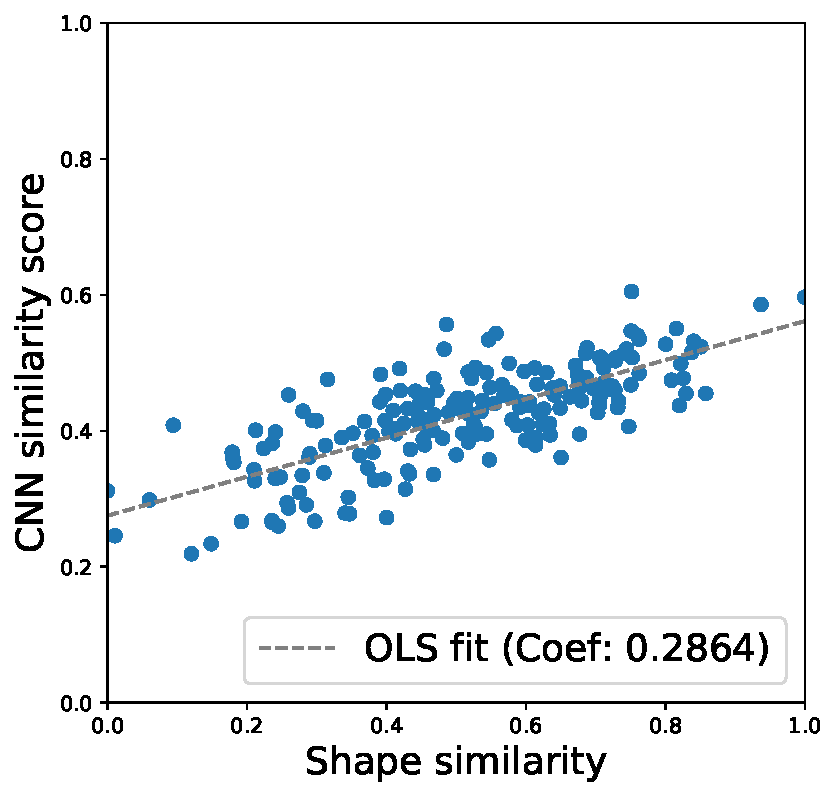
\includegraphics[width=\linewidth]{figures/vgg_shape_parametric.pdf}
%             \caption{Shape}
%         \end{subfigure}
%         \begin{subfigure}[b]{0.235\textwidth}
%             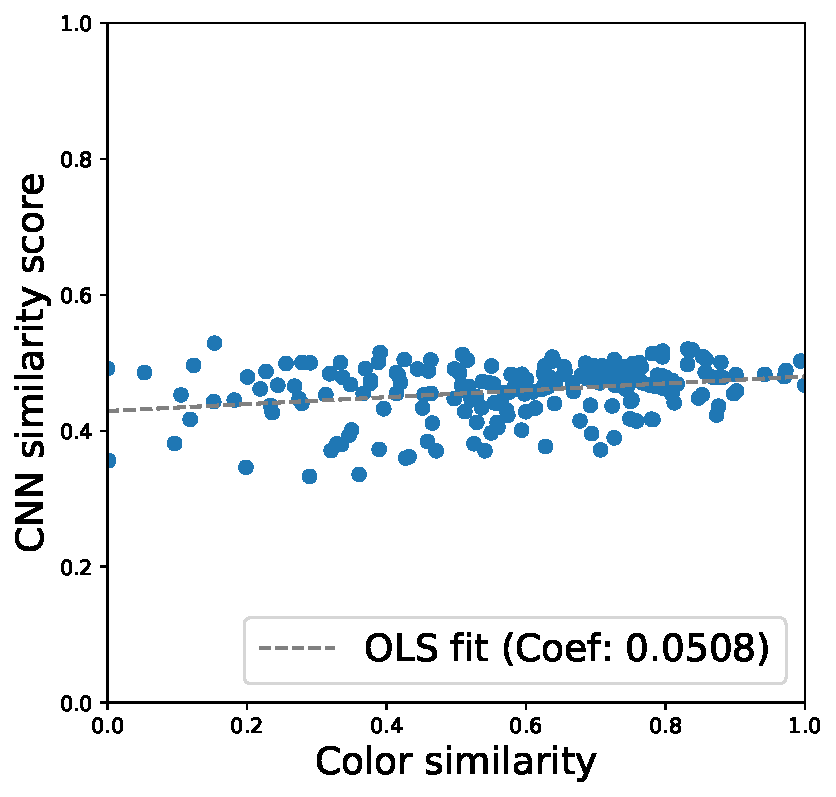
\includegraphics[width=\linewidth]{figures/vgg_color_parametric.pdf}
%             \caption{Color}
%         \end{subfigure}
%     \end{center}
%     \caption{VGG-16 parametric shape and color biases w/ other features varying.}
%     \label{fig:parametric_others_varying}
% \end{figure}